% Options for packages loaded elsewhere
\PassOptionsToPackage{unicode}{hyperref}
\PassOptionsToPackage{hyphens}{url}
%
\documentclass[
  doc, donotrepeattitle,floatsintext]{apa7}
\usepackage{amsmath,amssymb}
\usepackage{lmodern}
\usepackage{iftex}
\ifPDFTeX
  \usepackage[T1]{fontenc}
  \usepackage[utf8]{inputenc}
  \usepackage{textcomp} % provide euro and other symbols
\else % if luatex or xetex
  \usepackage{unicode-math}
  \defaultfontfeatures{Scale=MatchLowercase}
  \defaultfontfeatures[\rmfamily]{Ligatures=TeX,Scale=1}
\fi
% Use upquote if available, for straight quotes in verbatim environments
\IfFileExists{upquote.sty}{\usepackage{upquote}}{}
\IfFileExists{microtype.sty}{% use microtype if available
  \usepackage[]{microtype}
  \UseMicrotypeSet[protrusion]{basicmath} % disable protrusion for tt fonts
}{}
\makeatletter
\@ifundefined{KOMAClassName}{% if non-KOMA class
  \IfFileExists{parskip.sty}{%
    \usepackage{parskip}
  }{% else
    \setlength{\parindent}{0pt}
    \setlength{\parskip}{6pt plus 2pt minus 1pt}}
}{% if KOMA class
  \KOMAoptions{parskip=half}}
\makeatother
\usepackage{xcolor}
\usepackage{graphicx}
\makeatletter
\def\maxwidth{\ifdim\Gin@nat@width>\linewidth\linewidth\else\Gin@nat@width\fi}
\def\maxheight{\ifdim\Gin@nat@height>\textheight\textheight\else\Gin@nat@height\fi}
\makeatother
% Scale images if necessary, so that they will not overflow the page
% margins by default, and it is still possible to overwrite the defaults
% using explicit options in \includegraphics[width, height, ...]{}
\setkeys{Gin}{width=\maxwidth,height=\maxheight,keepaspectratio}
% Set default figure placement to htbp
\makeatletter
\def\fps@figure{htbp}
\makeatother
\setlength{\emergencystretch}{3em} % prevent overfull lines
\providecommand{\tightlist}{%
  \setlength{\itemsep}{0pt}\setlength{\parskip}{0pt}}
\setcounter{secnumdepth}{-\maxdimen} % remove section numbering
% Make \paragraph and \subparagraph free-standing
\ifx\paragraph\undefined\else
  \let\oldparagraph\paragraph
  \renewcommand{\paragraph}[1]{\oldparagraph{#1}\mbox{}}
\fi
\ifx\subparagraph\undefined\else
  \let\oldsubparagraph\subparagraph
  \renewcommand{\subparagraph}[1]{\oldsubparagraph{#1}\mbox{}}
\fi
\newlength{\cslhangindent}
\setlength{\cslhangindent}{1.5em}
\newlength{\csllabelwidth}
\setlength{\csllabelwidth}{3em}
\newlength{\cslentryspacingunit} % times entry-spacing
\setlength{\cslentryspacingunit}{\parskip}
\newenvironment{CSLReferences}[2] % #1 hanging-ident, #2 entry spacing
 {% don't indent paragraphs
  \setlength{\parindent}{0pt}
  % turn on hanging indent if param 1 is 1
  \ifodd #1
  \let\oldpar\par
  \def\par{\hangindent=\cslhangindent\oldpar}
  \fi
  % set entry spacing
  \setlength{\parskip}{#2\cslentryspacingunit}
 }%
 {}
\usepackage{calc}
\newcommand{\CSLBlock}[1]{#1\hfill\break}
\newcommand{\CSLLeftMargin}[1]{\parbox[t]{\csllabelwidth}{#1}}
\newcommand{\CSLRightInline}[1]{\parbox[t]{\linewidth - \csllabelwidth}{#1}\break}
\newcommand{\CSLIndent}[1]{\hspace{\cslhangindent}#1}
\ifLuaTeX
\usepackage[bidi=basic]{babel}
\else
\usepackage[bidi=default]{babel}
\fi
\babelprovide[main,import]{english}
% get rid of language-specific shorthands (see #6817):
\let\LanguageShortHands\languageshorthands
\def\languageshorthands#1{}
% Manuscript styling
\usepackage{upgreek}
\captionsetup{font=singlespacing,justification=justified}

% Table formatting
\usepackage{longtable}
\usepackage{lscape}
% \usepackage[counterclockwise]{rotating}   % Landscape page setup for large tables
\usepackage{multirow}		% Table styling
\usepackage{tabularx}		% Control Column width
\usepackage[flushleft]{threeparttable}	% Allows for three part tables with a specified notes section
\usepackage{threeparttablex}            % Lets threeparttable work with longtable

% Create new environments so endfloat can handle them
% \newenvironment{ltable}
%   {\begin{landscape}\centering\begin{threeparttable}}
%   {\end{threeparttable}\end{landscape}}
\newenvironment{lltable}{\begin{landscape}\centering\begin{ThreePartTable}}{\end{ThreePartTable}\end{landscape}}

% Enables adjusting longtable caption width to table width
% Solution found at http://golatex.de/longtable-mit-caption-so-breit-wie-die-tabelle-t15767.html
\makeatletter
\newcommand\LastLTentrywidth{1em}
\newlength\longtablewidth
\setlength{\longtablewidth}{1in}
\newcommand{\getlongtablewidth}{\begingroup \ifcsname LT@\roman{LT@tables}\endcsname \global\longtablewidth=0pt \renewcommand{\LT@entry}[2]{\global\advance\longtablewidth by ##2\relax\gdef\LastLTentrywidth{##2}}\@nameuse{LT@\roman{LT@tables}} \fi \endgroup}

% \setlength{\parindent}{0.5in}
% \setlength{\parskip}{0pt plus 0pt minus 0pt}

% Overwrite redefinition of paragraph and subparagraph by the default LaTeX template
% See https://github.com/crsh/papaja/issues/292
\makeatletter
\renewcommand{\paragraph}{\@startsection{paragraph}{4}{\parindent}%
  {0\baselineskip \@plus 0.2ex \@minus 0.2ex}%
  {-1em}%
  {\normalfont\normalsize\bfseries\itshape\typesectitle}}

\renewcommand{\subparagraph}[1]{\@startsection{subparagraph}{5}{1em}%
  {0\baselineskip \@plus 0.2ex \@minus 0.2ex}%
  {-\z@\relax}%
  {\normalfont\normalsize\itshape\hspace{\parindent}{#1}\textit{\addperi}}{\relax}}
\makeatother

% \usepackage{etoolbox}
\makeatletter
\patchcmd{\HyOrg@maketitle}
  {\section{\normalfont\normalsize\abstractname}}
  {\section*{\normalfont\normalsize\abstractname}}
  {}{\typeout{Failed to patch abstract.}}
\patchcmd{\HyOrg@maketitle}
  {\section{\protect\normalfont{\@title}}}
  {\section*{\protect\normalfont{\@title}}}
  {}{\typeout{Failed to patch title.}}
\makeatother

\usepackage{xpatch}
\makeatletter
\xapptocmd\appendix
  {\xapptocmd\section
    {\addcontentsline{toc}{section}{\appendixname\ifoneappendix\else~\theappendix\fi\\: #1}}
    {}{\InnerPatchFailed}%
  }
{}{\PatchFailed}
\keywords{Self-controlled, Knowledge of results, OPTIMAL theory, Retention}
\usepackage{csquotes}
\usepackage{pdflscape}
\usepackage{setspace}
\raggedbottom
\renewcommand\author[1]{}
\renewcommand\affiliation[1]{}
\authorsnames[1, 1, 1, 1, 1, 1, {2,3}, 1]{Laura St. Germain, Brad McKay, Andrew Poskus, Allison Williams, Olena Leshchyshen, Sherry Feldman, Joshua G.A. Cashaback, Michael J. Carter\vspace{2ex}}
\authorsaffiliations{{Department of Kinesiology, McMaster University}, {Department of Biomedical Engineering, University of Delaware}, {Interdisciplinary Neuroscience Graduate Program, University of Delaware}}
\ifLuaTeX
  \usepackage{selnolig}  % disable illegal ligatures
\fi
\IfFileExists{bookmark.sty}{\usepackage{bookmark}}{\usepackage{hyperref}}
\IfFileExists{xurl.sty}{\usepackage{xurl}}{} % add URL line breaks if available
\urlstyle{same} % disable monospaced font for URLs
\hypersetup{
  pdftitle={Exercising choice over feedback schedules during practice is not advantageous for motor learning},
  pdflang={en-EN},
  pdfkeywords={Self-controlled, Knowledge of results, OPTIMAL theory, Retention},
  hidelinks,
  pdfcreator={LaTeX via pandoc}}

\title{Exercising choice over feedback schedules during practice is not advantageous for motor learning}
\author{\phantom{0}}
\date{}


\shorttitle{Choice and feedback characteristics}

\authornote{

\vspace{-0.5cm}

\noindent \addORCIDlink{Laura St. Germain}{0000-0002-5513-4183} \newline
\noindent \addORCIDlink{Brad McKay}{0000-0002-7408-2323} \newline
\noindent \addORCIDlink{Joshua G.A. Cashaback}{0000-0002-8642-6648} \newline
\noindent \addORCIDlink{Michael J. Carter}{0000-0002-0675-4271}
\noindent Data and code: \url{https://github.com/cartermaclab/expt_sc-feedback-characteristics} \vspace{2ex} \newline
\noindent \textbf{Corresponding authors:} Michael J. Carter (\href{mailto:michaelcarter@mcmaster.ca}{\nolinkurl{michaelcarter@mcmaster.ca}}) and Laura St.~Germain (\href{mailto:stgerml@mcmaster.ca}{\nolinkurl{stgerml@mcmaster.ca}}).

}

\affiliation{\phantom{0}}

\abstract{%
The idea that there is a self-controlled learning advantage, where individuals demonstrate improved motor learning after exercising choice over an aspect of practice compared to no-choice groups, has different causal explanations according to the OPTIMAL theory or an information-processing perspective. Within OPTIMAL theory, giving learners choice is considered an autonomy-supportive manipulation that enhances expectations for success and intrinsic motivation. In the information-processing view, choice allows learners to engage in performance-dependent strategies that reduce uncertainty about task outcomes. To disentangle these potential explanations, we provided participants in choice and yoked groups with error or graded feedback (Experiment 1) and binary feedback (Experiment 2) while learning a rapid reaching task with spatial and timing goals. Across both experiments (N = 228 participants), we did not find evidence to support a self-controlled learning advantage. Exercising choice during practice did not increase perceptions of autonomy, competence, or intrinsic motivation, nor did it lead to more accurate error estimation skills. Both error and graded feedback facilitated skill acquisition and learning, whereas no improvements from pre-test performance were found with binary feedback. Finally, the impact of graded and binary feedback on perceived competence highlights a potential dissociation of motivational and informational roles of feedback. Although our results regarding self-controlled practice conditions are difficult to reconcile with either the OPTIMAL theory or the information-processing perspective, they are consistent with a growing body of evidence that strongly suggests self-controlled conditions are not an effective approach to enhance motor performance and learning.
}



\begin{document}
\maketitle

The underlying source of errors in skilled actions are often ambiguous and difficult to assign as the learner must rely on noisy and delayed sensory information. Feedback from an external source, such as a coach or computer display, can facilitate or augment this process (Sigrist et al., 2013). Knowledge of results feedback (Salmoni et al., 1984) can provide varying amounts of information to learners depending on its characteristics. Error feedback provides precise information about the magnitude and direction of the error (e.g., -42 cm), graded feedback provides coarse information about either the magnitude or direction of the error (e.g., ``too far''), and binary feedback indicates only success or failure information (e.g., ``miss'') (Luft, 2014). When to provide this feedback is often decided by an external agent; however, this feedback decision can also be made by the learner, a form of self-controlled learning. These self-controlled feedback schedules have typically enhanced motor skill learning compared to yoked feedback schedules, wherein learners experience the feedback schedule created by a self-controlled counterpart, but without any choice (see Sanli et al., 2013; Ste-Marie et al., 2020 for reviews).

Why self-controlled learning advantages emerge has garnered considerable attention in the motor skill learning literature. Within their OPTIMAL (Optimizing performance through intrinsic motivation and attentional learning) theory of motor learning, Wulf and Lewthwaite (2016) have argued that providing participants the opportunity to exercise choice, as in a self-controlled group, creates a virtuous cycle. Specifically, choice leads to increased (perceived) autonomy, leading to enhanced expectancies (e.g., perceived competence) and increased (intrinsic) motivation. These motivational influences lead to improved motor performance, creating a positive feedback loop that ultimately enhances motor learning compared to those not given the same choice opportunities. Support for this view has been drawn from experimental work where participants exercise choice over task-irrelevant or incidental choices. Exercising choice over the color of golf balls to putt (Lewthwaite et al., 2015 Experiment 1) or the mat underneath a target (Wulf et al., 2018 Experiment 1), which picture to hang in a lab (Lewthwaite et al., 2015 Experiment 2), hand order in a maximal force production task (Iwatsuki et al., 2017), which photos to look at while running (Iwatsuki et al., 2018), and the order of exercises to perform (Wulf et al., 2014) have been suggested to improve motor performance or learning. Other research, however, have failed to replicate this benefit of task-irrelevant or incidental choices on motor performance or learning (Carter \& Ste-Marie, 2017a; Grand et al., 2017; McKay \& Ste-Marie, 2020a, 2020b).

Rather than a motivational account, others have forwarded an information-processing explanation. From this perspective, exercising choice allows learners to tailor practice to their individual needs (Chiviacowsky \& Wulf, 2005, 2002) by engaging in performance-contingent strategies (Carter et al., 2014, 2016; Laughlin et al., 2015; Pathania et al., 2019) to reduce uncertainty about movement outcomes (Barros et al., 2019; Carter et al., 2014; Carter \& Ste-Marie, 2017a, 2017b; Grand et al., 2015). Evidence for this view has come from experiments that showed the timing of the feedback decision relative to task performance matters (Carter et al., 2014; Chiviacowsky \& Wulf, 2005), that task-relevant choices are more effective than task-irrelevant choices (Carter \& Ste-Marie, 2017a; cf. Wulf et al., 2018 Experiment 2), that interfering with information-processing activities during (Couvillion et al., 2020; Woodard \& Fairbrother, 2020) or after (Carter \& Ste-Marie, 2017b; Woodard \& Fairbrother, 2020) task performance eliminates self-controlled learning benefits, and that the ability to accurately estimate one's performance is enhanced in choice compared to yoked groups (Carter et al., 2014; Carter \& Patterson, 2012). Thus, further investigation is required to test predictions from these two explanations to better understand why exercising choice during practice confers an advantage for motor skill learning.

To dissociate between the motivational and information-processing accounts of the self-controlled learning advantage, we provided participants in choice and yoked (i.e., no-choice) groups with error or graded feedback (Experiment 1) and binary feedback (Experiment 2) during the acquisition of a rapid aiming task. Motor learning was assessed using delayed (\textasciitilde24 hours) retention and transfer tests. If the OPTIMAL theory is correct, we hypothesized that the characteristics of one's feedback schedule \emph{would not matter} for the self-controlled learning advantage as this advantage arises from the opportunity for choice--a common feature of all choice groups. Thus, we predicted all choice groups would demonstrate superior performance and learning compared to the yoked groups. Alternatively, if the information-processing account is correct, we hypothesized that the characteristics of one's feedback schedule \emph{would matter} for the self-controlled learning advantage as feedback with greater informational value would be more effective for reducing uncertainties about movement outcomes. Thus, we predicted that choice over an error feedback schedule would be the most effective pairing for performance and learning. We also included self-report measures of perceptions of autonomy, competence, and intrinsic motivation, and assessments of error estimation abilities to respectively test auxiliary assumptions of the OPTIMAL theory and information-processing explanations.

\hypertarget{methods}{%
\section{Methods}\label{methods}}

We report how we determined our sample size, all data exclusions (if any), all manipulations, and all measures in the study (Simmons et al., 2012). All data and \texttt{R} scripts can be accessed here: \url{https://github.com/cartermaclab/expt_sc-feedback-characteristics}.

\hypertarget{participants}{%
\subsection{Participants}\label{participants}}

\hypertarget{experiment-1}{%
\subsubsection{Experiment 1}\label{experiment-1}}

One hundred and fifty-two right-handed (Oldfield, 1971), healthy adults participated in Experiment 1 (\(M_{age}\) = 20.64 years, \(SD_{age}\) = 2.45, 88 females). Sample size was determined from an \emph{a-priori} power analysis using the \emph{ANOVA: fixed effects, main effects and interactions} option in G*Power (Faul et al., 2009) with the following parameters: \(\alpha\) = 0.05, \(\beta\) = .20, \(f\) = 0.23, numerator = 1, and groups = 2. This revealed a required sample of 151 participants. Our chosen effect size was based on a meta-analytic estimate (\(f\) = .32) by McKay et al. (2014); however, we used a more conservative estimate given the uncertainty of how choice would interact with our feedback characteristic manipulation. Participants were compensated \$15 CAD or with course-credit for their time. All participants gave written informed consent and the experiment was approved by McMaster University's Research Ethics Board.

\hypertarget{experiment-2}{%
\subsubsection{Experiment 2}\label{experiment-2}}

A new sample of 76 right-handed (Oldfield, 1971), healthy adults participated in Experiment 2 (\(M_{age}\) = 20.18 years, \(SD_{age}\) = 3.18, 47 females). Sample size was selected so group size matched that used in Experiment 1. Participants were compensated \$15 CAD or with course-credit for their time. All participants gave written informed consent and the experiment was approved by McMaster University's Research Ethics Board.

\hypertarget{task}{%
\subsection{Task}\label{task}}

In Experiments 1 and 2, participants sat in a chair facing a monitor (1920x1080 resolution) with their left arm in a custom manipulandum that restricted movement to the horizontal plane. Their elbow was bent at approximately 90° and they grasped a vertical handle with their left hand. Handle position was adjusted as needed to ensure the central axis of rotation was about the elbow. The task required a rapid ``out-and-back'' movement such that the reversal happened at \(40^\circ\) (in pre-test, acquisition, and retention) or \(60^\circ\) (in transfer). The starting point for all trials was \(0^\circ\). Participants were instructed to make a smooth movement to the reversal and back without hesitating when reversing their movement. The movement time goal to the reversal was always 225 ms. The task and instructions were similar to those used by Sherwood (1996; 2009). Vision of the manipulandum and limb were occluded during all phases of the experiment. Angular displacement for the elbow was collected via a potentiometer attached to the axis of rotation of the custom manipulandum. Potentiometer data were digitally sampled at 1000 Hz (National Instruments PCIe-6321) using a custom LabVIEW program and stored for offline analysis.

\hypertarget{procedure}{%
\subsection{Procedure}\label{procedure}}

\hypertarget{experiment-1-1}{%
\subsubsection{Experiment 1}\label{experiment-1-1}}

The first 76 participants were randomly assigned to either the Choice+Error-Feedback group (\(n\) = 38; \(M_{age}\) = 20.24 years, \(SD_{age}\) = 2.37, 22 females) or the Choice+Graded-Feedback group (\(n\) = 38; \(M_{age}\) = 20.76 years, \(SD_{age}\) = 3.02, 26 females). This is typical in the self-controlled learning literature as the self-controlled participants' self-selected feedback schedules are required for providing feedback to the participants in the yoked (i.e., control) groups. The remaining 76 participants were randomly assigned to either the Yoked+Error-Feedback group (\(n\) = 38; \(M_{age}\) = 20.53 years, \(SD_{age}\) = 2.13, 23 females) or the Yoked+Graded-Feedback group (\(n\) = 38; \(M_{age}\) = 21.03 years, \(SD_{age}\) = 2.32, 22 females).

Data collection consisted of two sessions separated by approximately 24 hours.\footnote{Six participants (three Choice+Error-Feedback and three Choice+Graded-Feedback) had their second session completed approximately 48 hours later because a snowstorm closed the University.} Session one included a pre-test (12 trials) and an acquisition phase (72 trials). Session two included the delayed retention (12 trials) and transfer (12 trials) tests. No feedback about motor performance was provided in pre-test, retention, or transfer. Prior to the pre-test, all participants received instructions about the task and its associated spatial and timing goals. Additionally, half of the participants in each group were randomly selected to estimate their performance on the spatial and timing goals after each trial in the pre-test. Only a subset of participants were asked to estimate their performance in pre-test to mitigate the potential that doing so would prompt participants to adopt this strategy during the experiment as error estimation has been suggested (e.g., Chiviacowsky \& Wulf, 2005) to be adopted spontaneously by participants controlling their feedback schedule. However, asking participants to estimate their performance during pre-test is necessary to be able to assess how this skill develops as a function of one's practice condition.

Participants were reminded of the instructions about the task and its associated goals at the start of the acquisition phase. Group specific instructions regarding feedback were also provided. Participants in the Choice+Error-Feedback group and the Choice+Graded-Feedback group were told they could choose their feedback schedule, with the restriction that they must select feedback on 24 of the 72 acquisition trials. They were informed that if the number of remaining feedback requests equaled the number of remaining acquisition trials, these trials would default to feedback trials. This feedback restriction was implemented to ensure the relative frequency of feedback was equated across all groups. Similar restrictions have been used in past research involving multiple choice groups (e.g., Chiviacowsky \& Wulf, 2005). Participants in the Yoked+Error-Feedback group and the Yoked+Graded-Feedback group were told they may or may not receive feedback following a trial based on a predetermined schedule. Thus, participants in these groups were not aware that their feedback schedule was actually created by a participant in a corresponding choice group. While this yoking procedure ensures that the total number of feedback trials and their relative placement during acquisition are identical, the content of the feedback reflected each participant's own performance. Error feedback for the spatial and timing goals was provided as the difference between the participant's actual performance and the task goal (i.e., constant error). Graded feedback for the spatial goal was provided as ``too short'' if performance was \textless{} 40 degrees (or 60 degrees in transfer), ``hit'' if exactly 40 degrees, and ``too far'' if \textgreater{} 40 degrees. For the timing goal, graded feedback was provided as ``too fast'' when performance was \textless{} 225 ms, ``hit'' if exactly 225 ms, and ``too slow'' if \textgreater{} 225 ms. All participants were shown a sample feedback display that corresponded to their experimental group and were asked to interpret it aloud for the researcher to verify understanding.

\begin{figure}

{\centering 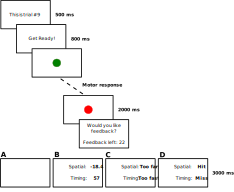
\includegraphics[height=0.45\textheight]{../../figs/fig1} 

}

\caption{\small \onehalfspacing \textbf{Overview of a typical acquisition trial for the choice groups.} The sequence of events a participant in the choice groups experienced during the acquisition phase. Trials began by informing participants the trial number (500 ms) they were on in acquisition. Shortly after, the text ``Get Ready!'' appeared on the screen and 800 ms later a visual go-signal was presented in the form of a green circle in the center of the screen. Participants began their movement when ready after seeing the visual go-signal as we were not interested in reaction time. While participants completed their rapid out-and-back movement, the computer screen was blank. Upon returning to the starting position, a red circle appeared in the center of the screen. A 2000 ms feedback delay interval was used and this interval was followed by the feedback prompt. The feedback prompt also displayed an updated counter representing the number of feedback trials they had left. If the number of remaining feedback trials matched the number of acquisition trials left, these trials automatically defaulted to feedback trials. On trials where feedback was not requested, a blank screen \textbf{(A)} was shown for 3000 ms. When feedback was selected, feedback was provided for both the spatial and timing goals according to their experimental group. The error feedback group \textbf{(B)} saw their constant error, the graded feedback group \textbf{(C)} saw either ``too far'' or ``too short'' for the spatial goal and ``too fast'' or ``too slow'' for the timing goal, and the binary feedback group \textbf{(D)} saw either ``hit'' or ``miss'' for the task goals. The sequence of events was the same for the yoked groups with the exception they did not see a feedback prompt. The sequence of events was similar in pre-test, retention, and transfer except all trials were no-feedback trials.}\label{fig:fig1}
\end{figure}



A typical acquisition trial (see Figure \ref{fig:fig1}) began with the current trial number displayed (500 ms), followed by a visual ``Get Ready!'' and a visual go-signal (800 ms apart). Participants were free to begin their movement when ready following the visual go-signal (i.e., green circle) as this was not a reaction time task. The computer screen was blank while participants made their movement. When participants returned to the starting position, a red circle was displayed on the monitor. Following a 2000 ms feedback delay interval, the feedback decision prompt was presented for the self-controlled groups. If feedback was not selected, a blank screen was displayed for 3000 ms. If feedback was selected (or imposed on the yoked groups), it was also displayed for 3000 ms.

Before the retention and transfer tests, participants were reminded about the task and its associated goals. All participants were asked to estimate their performance after each trial in retention and transfer. After the pre-test, trials 12 and 72 in acquisition, and before the delayed retention test, participants answered a series of questions pertaining to perceived competence, task interest and enjoyment, and perceived autonomy. The perceived competence and task interest and enjoyment questions were from the Intrinsic Motivation Inventory (McAuley et al., 1989; Ryan, 1982) and the perceived autonomy questions were used in earlier work (Barros et al., 2019; Carter \& Ste-Marie, 2017a). Cronbach's alpha values for each questionnaire at each time point are reported in Table \ref{tab:table1}.

\hypertarget{experiment-2-1}{%
\subsubsection{Experiment 2}\label{experiment-2-1}}

Similar to Experiment 1, the first half of participants were assigned to the Choice+Binary-Feedback group (\(n\) = 38; \(M_{age}\) = 22.37 years, \(SD_{age}\) = 3.13, 19 females) and the remaining participants were assigned to the Yoked+Binary-Feedback group (\(n\) = 38; \(M_{age}\) = 18.00 years, \(SD_{age}\) = 0.93, 28 females). Binary feedback for the spatial goal was provided as ``hit'' if performance was exactly 40 degrees (or 60 degrees in transfer) and as ``miss'' for everything else. For the timing goal, binary feedback was provided as ``hit'' when performance was exactly 225 ms and as ``miss'' for everything else. Data collection was identical to that of Experiment 1, except in the acquisition instructions participants in both groups were shown a sample binary feedback display and were asked to interpret it aloud for the researcher to verify understanding.

\begin{table}

\caption{\label{tab:table1}Cronbach's alpha for each questionnaire at each timepoint.}
\fontsize{11}{13}\selectfont
\begin{tabular}[t]{>{\raggedright\arraybackslash}p{12em}>{\raggedright\arraybackslash}p{6em}>{\raggedright\arraybackslash}p{6em}>{\raggedright\arraybackslash}p{6em}>{\raggedright\arraybackslash}p{7em}}
\toprule
Questionnaire & After pre-test & After block 1 & After block 6 & Before retention\\
\midrule
\addlinespace[0.3em]
\multicolumn{5}{l}{\textbf{Experiment 1}}\\
\hspace{1em}Perceived autonomy & 0.68 & 0.81 & 0.80 & 0.83\\
\hspace{1em}Perceived competence & 0.86 & 0.93 & 0.95 & 0.94\\
\hspace{1em}Intrinsic motivation & 0.86 & 0.90 & 0.92 & 0.93\\
\addlinespace[0.3em]
\multicolumn{5}{l}{\textbf{Experiment 2}}\\
\hspace{1em}Perceived autonomy & 0.39 & 0.73 & 0.79 & 0.85\\
\hspace{1em}Perceived competence & 0.92 & 0.88 & 0.91 & 0.91\\
\hspace{1em}Intrinsic motivation & 0.91 & 0.91 & 0.93 & 0.94\\
\bottomrule
\multicolumn{5}{l}{\rule{0pt}{1em}\textit{Note.} Block 1 and 6 are from the acquisition phase.}\\
\end{tabular}
\end{table}

\hypertarget{data-analysis}{%
\subsection{Data Analysis}\label{data-analysis}}

Movement trajectories for all trials were visually inspected by a researcher and trials with errors (e.g., technical issues, moving before the ``go'' signal) were removed. A total of 4.03\% (662/16146) and 3.73\% (306/8208) of trials for Experiments 1 and 2 were removed, respectively. Trials were aggregated into blocks of 12 trials, resulting in one block of trials for pre-test, retention, and transfer, and six blocks of trials for acquisition. Our primary performance outcome variable was total error (E) (Henry, 1974, 1975) and was computed using the equation:
\begin{equation}
E = \sqrt{\sum{(x_{i} - T)^2 / n}}
\end{equation}
where \(x_{i}\) is the score on the \(i\)th trial, \(T\) is the target goal, and \(n\) is the number of trials in a block.

To test for performance differences in pre-test, retention, and transfer, total error for the spatial and timing goals were analyzed in separate mixed ANOVAs (\emph{Experiment 1:} 2 Choice x 2 Feedback x 3 Test; \emph{Experiment 2:} 2 Choice x 3 Test). To test for performance differences during acquisition, total error for the spatial and timing goals during acquisition were analyzed in separate mixed ANOVAs (\emph{Experiment 1:} 2 Choice x 2 Feedback x 6 Block; \emph{Experiment 2:} 2 Choice x 6 Block). Our primary psychological outcome variables were intrinsic motivation (i.e., interest/enjoyment), perceived competence, and perceived autonomy. The mean score of the responses for these constructs at each time point was calculated for each participant and analyzed in separate mixed ANOVAs (\emph{Experiment 1:} 2 Choice x 2 Feedback x 4 Time; \emph{Experiment 2:} 2 Choice x 4 Time). Of secondary interest, error estimation abilities were assessed as total error between a participant's estimation and actual performance in pre-test (50\% of the participants in each group in Experiments 1 and 2), retention, and transfer (see \textbf{Supplementary A}).

Alpha was set to .05 for all statistical analyses. Corrected degrees of freedom using the Greenhouse-Geisser technique are always reported for repeated measures with more than two levels. Generalized eta squared \((\eta_{G}^2)\) is provided as an effect size statistic (Bakeman, 2005; Lakens, 2013; Olejnik \& Algina, 2003) for all omnibus tests. Post hoc comparisons were Holm-Bonferroni corrected to control for multiple comparisons. Statistical tests were conducted using R (Version 4.1.2; R Core Team, 2021) and the R-packages \emph{afex} (Version 1.1.1; Singmann et al., 2021), \emph{computees} (Re, 2013), \emph{ggResidpanel} (Version 0.3.0.9000; Goode \& Rey, 2022), \emph{kableExtra} (Version 1.3.4; Zhu, 2021), \emph{metafor} (Version 3.4.0; Viechtbauer, 2010), \emph{papaja} (Version 0.1.0.9999; Aust \& Barth, 2020), \emph{patchwork} (Version 1.1.0.9000; Pedersen, 2020), \emph{rogme} (Version 0.2.1; Rousselet et al., 2017), \emph{tidyverse} (Version 1.3.1; Wickham et al., 2019), and \emph{tinylabels} (Version 0.2.3; Barth, 2022) were used in this project.

\hypertarget{results}{%
\section{Results}\label{results}}

Model diagnostics of total error for the spatial and timing goals revealed skewed distributions. We therefore conducted sensitivity analyses using the shift function, which is a robust statistical method well-suited for skewed distributions (Rousselet \& Wilcox, 2020; Wilcox, 2021). The results of these analyses (see \textbf{Supplementary B}) were consistent with those of the mixed ANOVAs, which we report below.

\hypertarget{pre-test-retention-and-transfer}{%
\subsection{Pre-test, retention, and transfer}\label{pre-test-retention-and-transfer}}

\hypertarget{experiment-1-2}{%
\subsubsection{Experiment 1}\label{experiment-1-2}}

Spatial (Fig. \ref{fig:fig2}A) and timing (Fig. \ref{fig:fig2}B) error decreased from the pre-test to the retention and transfer tests. There was a main effect of Test for spatial error, \(F(1.33,196.52) = 40.20\), \(p < .001\), \(\eta_{G}^2 = .138\), where performance was less errorful in retention and transfer than pre-test (\(p\)'s \textless{} .001) and performance in retention was better than transfer (\(p\) \textless{} .001). A main effect of Test was also found for timing error, \(F(1.08,160.23) = 81.21\), \(p < .001\), \(\eta_{G}^2 = .245\), with pre-test performance more errorful than both retention and transfer (\(p\)'s \textless{} .001), and retention was less errorful than transfer (\(p\) \textless{} .001).

\hypertarget{experiment-2-2}{%
\subsubsection{Experiment 2}\label{experiment-2-2}}

Spatial (Fig. \ref{fig:fig3}A) and timing (Fig. \ref{fig:fig3}B) error did not change considerably from the pre-test to the retention and transfer tests. There were no significant main effects or interactions for either task goals.

\vspace{4ex}

\begin{figure}

{\centering \includegraphics{../../figs/fig2} 

}

\caption{\small \onehalfspacing \textbf{Experiment 1 data.} The Choice with error feedback (Choice+Error) group is shown in dark blue circles, the Choice with graded feedback (Choice+Graded) group is shown in light blue squares, the Yoked with error feedback (Yoked+Error) group is shown in red triangles, and the Yoked with graded feedback (Yoked+Graded) group is shown in yellow crosses. Error bars denote 95\% bootstrapped confidence intervals. \textbf{(A)} Spatial total error (degrees) and \textbf{(B)} timing total error (ms) averaged across blocks and participants within each group. Dotted vertical lines denote the different experimental phases. Pre-test and acquisition occurred on Day 1 and retention and transfer occurred approximately 24-hours later on Day 2. Self-reported scores for perceived autonomy \textbf{(C)}, perceived competence \textbf{(D)}, and intrinsic motivation \textbf{(E)} after the pre-test and after blocks 1 and 6 of acquisition on Day 1, and before the retention test on Day 2. Scores could range on a Likert scale from 1 (Strongly disagree) to 7 (Strongly agree). Dots represent individual data points.}\label{fig:fig2}
\end{figure}



\begin{figure}

{\centering \includegraphics{../../figs/fig3} 

}

\caption{\small \onehalfspacing \textbf{Experiment 2 data.} The Choice with binary feedback (Choice+Binary) group is shown in green circles and the Yoked with binary feedback (Yoked+Binary) group is shown in purple squares. Error bars denote 95\% bootstrapped confidence intervals. \textbf{(A)} Spatial total error (degrees) and \textbf{(B)} timing total error (ms) averaged across blocks and participants within each group. Dotted vertical lines denote the different experimental phases. Pre-test and acquisition occurred on Day 1 and retention and transfer occurred approximately 24-hours later on Day 2. Self-reported scores for perceived autonomy \textbf{(C)}, perceived competence \textbf{(D)}, and intrinsic motivation \textbf{(E)} after the pre-test and after blocks 1 and 6 of acquisition on Day 1, and before the retention test on Day 2. Scores could range on a Likert scale from 1 (Strongly disagree) to 7 (Strongly agree). Dots represent individual data points.}\label{fig:fig3}
\end{figure}



\newpage

\hypertarget{acquisition}{%
\subsection{Acquisition}\label{acquisition}}

\hypertarget{experiment-1-3}{%
\subsubsection{Experiment 1}\label{experiment-1-3}}

All groups of participants improved their performance of the spatial goal during the acquisition phase (Fig. \ref{fig:fig2}A). This was supported by a significant main effect of Block, \(F(2.41,357.13) = 60.18\), \(p < .001\), \(\eta_{G}^2 = .130\), where block 1 was less accurate than all other blocks (\(p\)'s \(< .001\)), block 2 was less accurate than all subsequent blocks (\(p\)'s \(\leq .021\)), and blocks 3 and 4 were more errorful than block 6 (\(p\)'s \(\leq .015\)). Timing error also decreased during the acquisition period (Fig. \ref{fig:fig2}B). The significant main effect of Block, \(F(1.75,259.59) = 55.44\), \(p < .001\), \(\eta_{G}^2 = .138\), was superseded by a significant Feedback x Block interaction, \(F(1.75, 259.59) = 3.56\), \(p = .035\), \(\eta_{G}^2 = .010\). Post hoc comparisons showed that timing error for those receiving error feedback was reduced from block 1 in all subsequent blocks (\(p\)'s \(< .001\)), but performance plateaued from block 2 onward in acquisition (\(p\)'s \(\geq .257\)). Timing error for the participants that received graded feedback was also reduced from block 1 in all subsequent blocks (\(p\)'s \(< .001\)); however, these participants continued to improve across acquisition blocks as block 2 was more errorful than blocks 3 to 6 (\(p\)'s \(\leq .028\)).

\hypertarget{experiment-2-3}{%
\subsubsection{Experiment 2}\label{experiment-2-3}}

Spatial (Fig. \ref{fig:fig3}A) and timing (Fig. \ref{fig:fig3}B) error remained relatively flat from block 1 to block 6 in the acquisition period. None of the main effects or interactions for either task goals were significant.

\hypertarget{psychological-variables}{%
\subsection{Psychological variables}\label{psychological-variables}}

\hypertarget{experiment-1-4}{%
\subsubsection{Experiment 1}\label{experiment-1-4}}

Perceptions of autonomy (Fig. \ref{fig:fig2}C) showed a slight decrease across time points, supported by a main effect of Time, \(F(2.25,332.95) = 3.69\), \(p < .022\), \(\eta_{G}^2 = .003\). Perceived autonomy was higher after block 1 of acquisition compared to self-reported ratings prior to completing the retention test (\(p = .031\)). Self-ratings for perceived competence (Fig. \ref{fig:fig2}D) were similar across groups after the pre-test, but then began to diverge after block 1 based on feedback characteristic. Main effects of Time, \(F(1.92, 283.47) = 3.43\), \(p = .036\), \(\eta_{G}^2 = .006\), and Feedback, \(F(1,148) = 47.36\), \(p < .001\), \(\eta_{G}^2 = .188\), were superseded by a Feedback x Time interaction, \(F(1.92, 283.47) = 28.04\), \(p < .001\), \(\eta_{G}^2 = .050\). Perceived competence scores were not significantly different after the pre-test (\(p = .232\)); however, perceptions of competence were significantly lower in those participants receiving graded feedback compared to error feedback at all other time points (\(p\)'s \(< .001\)). Self-reported scores for intrinsic motivation (Fig. \ref{fig:fig2}E) generally decreased after block 1, which was supported by a main effect of Time, \(F(2.40,355.90) = 14.69\), \(p < .001\), \(\eta_{G}^2 = .012\). Intrinsic motivation scores initially increased following the pre-test to after block 1 (\(p = .003\)); however, scores after block 1 of acquisition were greater than those reported at the end of acquisition (i.e., block 6) and before retention (\(p\)'s \(< .001\)). Self-reported ratings were also lower before retention compared to after the pre-test (\(p = .043\)).

\hypertarget{experiment-2-4}{%
\subsubsection{Experiment 2}\label{experiment-2-4}}

Self-reported scores for perceived autonomy (Fig. \ref{fig:fig3}C) were similar across all time points. There were no main effects or interactions. Perceptions of competence (Fig. \ref{fig:fig3}D) showed a considerable decrease after the pre-test, \(F(1.85,136.91) = 106.10\), \(p < .001\), \(\eta_{g}^2 = .298\), where scores were significantly greater after the pre-test compared to all other time points (\(p\)'s \(< .001\)), and were higher after block 1 of acquisition than before retention (\(p = .004\)). Self-ratings for intrinsic motivation generally decreased across time points, which was supported by a main effect of Time, \(F(2.37,175.55) = 15.31\), \(p < .001\), \(\eta_{G}^2 = .018\). Intrinsic motivation was higher after the pre-test than after block 6 of acquisition and before retention (\(p\)'s \(< .001\)), and higher after block 1 than after block 6 and before retention (\(p\)'s \(< .026\)).

\hypertarget{equivalence-analysis}{%
\subsection{Equivalence analysis}\label{equivalence-analysis}}

Our main comparison of interest was between choice and no-choice (i.e., yoked groups). To evaluate the self-controlled learning effect observed across Experiments 1 and 2, Hedges' \emph{g} for the spatial and timing goals were aggregated within each experiment while accounting for within-subject dependencies. Next, a random effects meta-analysis was conducted on the retention test data\footnote{We report an estimate for retention tests to facilitate comparison to a recent meta-analysis (McKay et al., in-press) that produced estimated effects of self-controlled learning at retention specifically.} to generate a summary point estimate and 90\% confidence intervals (CI). This resulted in an overall estimated effect of \(g = .05\) (favoring self-controlled) and \(90\% \,CI \,[-.12,.23]\).

Equivalence tests can be conducted to evaluate whether the observed differences are significantly smaller than a pre-determined smallest effect size of interest (see Harms \& Lakens, 2018 for a discussion). Typically, a two one-sided tests procedure is used to compare the observed effect to upper and lower equivalence bounds, and if the effect is significantly smaller than both bounds then the hypothesis that the effect is large enough to be of interest is rejected (Lakens, 2017; Schuirmann, 1987). However, we did not pre-specify a smallest effect of interest, so instead we report the 90\% confidence intervals (see above). All effect sizes outside this interval would be rejected by the two-one sided tests procedure while all values inside the interval would not. Therefore, the present experiments can be considered inconsistent with all effects larger than \(g = \pm.23\).

\hypertarget{discussion}{%
\section{Discussion}\label{discussion}}

The purpose of the present experiments was to test between motivational and information-processing accounts of the putative self-controlled learning advantage (see Ste-Marie et al., 2020 for a review). According to the OPTIMAL theory (Wulf \& Lewthwaite, 2016), self-controlled practice or choice conditions are advantageous because the provision of choice increases perceptions of autonomy and competence, which increase intrinsic motivation and ultimately both motor performance and learning. Conversely, others have argued that self-controlled feedback is effective because it provides the opportunity to request feedback in a performance dependent way that reduces uncertainty about movement outcomes relative to task goals (Carter et al., 2014; Carter \& Ste-Marie, 2017b; Grand et al., 2015). In contrast to these predictions, we did not find evidence that providing learners with choice over their feedback schedule was beneficial for motor learning, despite collecting a much larger sample (\emph{N} = 228 across both Experiments) than those commonly used in self-controlled learning experiments (median sample size \emph{N} = 36 in a meta-analysis by McKay et al., in-press) and motor learning experiments in general (median \emph{n}/group = 11 in a review by Lohse et al., 2016). Further, exercising choice in practice did not enhance perceptions of autonomy, competence, or intrinsic motivation, and also did not result in more accurate performance estimations in delayed tests of motor learning. Overall, we found no support for the OPTIMAL theory or information-processing perspective. Our results challenge the prevailing view that the self-controlled learning benefit is a robust effect.

The failed replication of a self-controlled learning advantage was surprising given the dominant view for the past 25 years has been that it is a robust effect and one that should be recommended to coaches and practitioners (Sanli et al., 2013; Ste-Marie et al., 2020; Wulf \& Lewthwaite, 2016). Our findings are, however, consistent with a growing list of relatively large--often pre-registered--experiments that have not found self-controlled learning benefits (Bacelar et al., 2022; Grand et al., 2017; Leiker et al., 2019; McKay \& Ste-Marie, 2020a, 2020b; St Germain et al., in-press; Yantha et al., in-press). One possible explanation for this discrepancy between earlier and more recent experiments may be that the self-controlled learning advantage was the result of underpowered designs, which has been highlighted as a problem in motor learning research (see Lohse et al., 2016 for a discussion). When underpowered designs find significant results, they are prone to be false positives with inflated estimates of effects (Button et al., 2013; Lakens \& Evers, 2014), which can be further exaggerated with questionable research practices such as \emph{p}-hacking and selective reporting (e.g., Munafò et al., 2017; Simmons et al., 2011). Thus, a self-controlled learning advantage may not actually exist. Alternatively, if one does exist then it seems likely it is a much smaller effect than originally estimated and requires considerably larger samples to reliability detect than those commonly used in motor learning research. Consistent with these ideas, a recent meta-analysis provided compelling evidence that the self-controlled learning advantage is not robust and its prominence in the motor learning literature is due to selective publication of statistically significant results (McKay et al., in-press). We estimated the overall effect of self-controlled practice in retention to be significantly smaller than any effect larger than \(g = .23\). This is consistent with the estimates from McKay et al. (in-press) after accounting for publication bias (\(g =\) -.11 to .26), which suggested either no effect or a small effect in an unknown direction. Taken together, we argue that it may be time for the self-controlled learning advantage to be considered a non-replicable effect in motor learning.

Given our current replication failure with those in recent years (Bacelar et al., 2022; Grand et al., 2017; Leiker et al., 2019; McKay \& Ste-Marie, 2020a, 2020b; St Germain et al., in-press; Yantha et al., in-press) and the conclusions from McKay et al. (in-press), motivational (i.e., OPTIMAL theory) versus information-processing explanations seem moot. Nevertheless, the present results are incompatible with both perspectives. Specifically, having choice opportunities during practice did not enhance perceptions of autonomy, competence, or intrinsic motivation in either experiment, inconsistent with OPTIMAL theory. Similarly, self-controlled feedback schedules did not enhance error estimation skills (see \textbf{Supplementary A}) and choice did not interact with feedback characteristics, inconsistent with the information-processing perspective. Instead, the results from Experiments 1 and 2 suggest that feedback characteristics were a more important determinant of motor performance during acquisition and delayed tests of learning than the opportunity to choose. When feedback provided information about the direction of an error or when it contained both direction and magnitude of an error, participants were able to improve at the task throughout acquisition and retain these improvements in skill relative to pre-test. However, when feedback was binary and direction and magnitude of an error was absent, there was no improvement in skill from baseline levels. This is in contrast with past research that has shown people can learn motor tasks with binary feedback (e.g., Cashaback et al., 2017, 2019; Izawa \& Shadmehr, 2011). One possible explanation for this discrepancy may be the amount of practice trials (Magill \& Wood, 1986). Practicing with binary feedback may inherently require a longer training period for learning to occur compared to graded and error feedback, which both have greater precision. Additionally, we used a strict criteria with binary feedback where any outcome other than zero error was considered a miss. Thus, binary feedback may be more effective when paired with a tolerance zone such as that used in the bandwidth technique (see Anderson et al., 2020 for a review; Cauraugh et al., 1993; Lee \& Carnahan, 1990).

Although unexpected, the influence of feedback characteristics on perceptions of competence may hint to a dissociation between informational and motivational impacts of knowledge-of-results feedback. In Experiment 1, participants who received graded feedback reported significantly lower perceptions of competence than participants who received error feedback. Yet, despite these lower expectations for success, the graded feedback groups did not demonstrate degraded performance or learning compared to the error feedback group. Participants in Experiment 2 who received binary feedback reported the lowest perceptions of competence and were also the only participants who did not show improvements in task performance from pre-test. Thus, future research is necessary to better understand this dissociation of informational and motivational influences of feedback characteristics and how it interacts with the task, individual, and environment.

In two experiments we failed to observe the predicted benefits of self-controlled feedback on motor learning. Similarly, we failed to find the predicted motivational and informational consequences of choice in either experiment, challenging both the OPTIMAL theory and information-processing explanation of the so-called self-controlled learning advantage. Although the present experiments were not pre-registered, the analysis plan was determined prior to viewing the data. In addition, a suite of sensitivity analyses were conducted to determine the extent to which the present results depended on the chosen analysis methods (see \textbf{Supplementary B}). The sensitivity analyses supported the conclusions of the primary analyses and are consistent with research that has followed pre-registered analysis plans (Bacelar et al., 2022; Grand et al., 2017; Leiker et al., 2019; McKay \& Ste-Marie, 2020a, 2020b; St Germain et al., in-press; Yantha et al., in-press). Lastly, our results and conclusions are in line with a recent meta-analysis (McKay et al., in-press) that suggests the apparent benefits of self-controlled practice are due to selection bias rather than true effects.

\vspace{2.5ex}

\hypertarget{funding}{%
\section{Funding}\label{funding}}

This work was supported by the Natural Sciences and Engineering Research Council (NSERC) of Canada (RGPIN-2018-05589; MJC) and McMaster University. LSG was supported by an NSERC Postgraduate Scholarship. JGAC was supported by an NIH U45GM104941 grant. AW and AP were supported by NSERC Undergraduate Student Research Awards.

\hypertarget{conflicts-of-interestcompeting-interests}{%
\section{Conflicts of interest/Competing interests}\label{conflicts-of-interestcompeting-interests}}

None.

\hypertarget{availability-of-data-materials-and-code}{%
\section{Availability of data, materials, and code}\label{availability-of-data-materials-and-code}}

Can be accessed here: \url{https://github.com/cartermaclab/expt_sc-feedback-characteristics}.

\hypertarget{authors-contributions-using-credit}{%
\section{Authors' contributions using CRediT}\label{authors-contributions-using-credit}}

Laura St.~Germain served as lead for data curation, formal analysis,investigation - performed experiment, project administration, and software - task programming, writing - original draft preparation, and writing - review and editing, contributed equally to conceptualization, methodology, validation, and visualization. Brad McKay contributed equally to conceptualization, methodology, validation, visualization, writing - original draft preparation, and writing - review and editing. Andrew Poskus served as a lead for investigation - performed experiment and served in a supporting role for writing- original draft preparation and writing - review and editing. Allison Williams served as a lead for investigation - performed experiment and served in a supporting role for writing - original draft preparation and writing - review and editing. Olena Leshchyshen contributed equally to investigation - performed experiment and served in a supporting role for writing - original draft preparation and writing - review and editing. Sherry Feldman contributed equally to investigation - performed experiment and served in a supporting role for writing - original draft preparation and writing - review and editing. Joshua G.A. Cashaback contributed equally to conceptualization, methodology, writing - original draft preparation, and writing - review and editing. Michael J. Carter served as lead for funding acquisition, resources, and supervision, contributed equally to conceptualization, methodology, validation, visualization, writing - original draft preparation, and writing - review and editing, and served in a supporting role for data curation, formal analysis, project administration, and software - task programming.

\hypertarget{references}{%
\section{References}\label{references}}

\vspace{2ex}

\hypertarget{refs}{}
\begin{CSLReferences}{1}{0}
\leavevmode\vadjust pre{\hypertarget{ref-anderson2020}{}}%
Anderson, D. I., Magill, R. A., Mayo, A. M., \& Steel, K. A. (2020). Enhancing motor skill acquisition with augmented feedback. In \emph{Skill acquisition in sport: Research, theory and practice} (3rd ed.). {Routledge}.

\leavevmode\vadjust pre{\hypertarget{ref-R-papaja}{}}%
Aust, F., \& Barth, M. (2020). \emph{{papaja}: {Prepare} reproducible {APA} journal articles with {R Markdown}}. \url{https://github.com/crsh/papaja}

\leavevmode\vadjust pre{\hypertarget{ref-bacelar2022}{}}%
Bacelar, M. F. B., Parma, J. O., Cabral, D., Daou, M., Lohse, K. R., \& Miller, M. W. (2022). Dissociating the contributions of motivational and information processing factors to the self-controlled feedback learning benefit. \emph{Psychology of Sport and Exercise}, \emph{59}, 102119. \url{https://doi.org/10.1016/j.psychsport.2021.102119}

\leavevmode\vadjust pre{\hypertarget{ref-bakeman2005}{}}%
Bakeman, R. (2005). Recommended effect size statistics for repeated measures designs. \emph{Behavior Research Methods}, \emph{37}(3), 379--384. \url{https://doi.org/10.3758/bf03192707}

\leavevmode\vadjust pre{\hypertarget{ref-barros2019}{}}%
Barros, J. A. C., Yantha, Z. D., Carter, M. J., Hussien, J., \& Ste-Marie, D. M. (2019). Examining the impact of error estimation on the effects of self-controlled feedback. \emph{Human Movement Science}, \emph{63}, 182--198. \url{https://doi.org/10.1016/j.humov.2018.12.002}

\leavevmode\vadjust pre{\hypertarget{ref-R-tinylabels}{}}%
Barth, M. (2022). \emph{{tinylabels}: Lightweight variable labels}. \url{https://cran.r-project.org/package=tinylabels}

\leavevmode\vadjust pre{\hypertarget{ref-button2013}{}}%
Button, K. S., Ioannidis, J. P. A., Mokrysz, C., Nosek, B. A., Flint, J., Robinson, E. S. J., \& Munafò, M. R. (2013). Power failure: why small sample size undermines the reliability of neuroscience. \emph{Nature Reviews Neuroscience}, \emph{14}(5), 365--376. \url{https://doi.org/10.1038/nrn3475}

\leavevmode\vadjust pre{\hypertarget{ref-carter2014}{}}%
Carter, M. J., Carlsen, A. N., \& Ste-Marie, D. M. (2014). Self-controlled feedback is effective if it is based on the learner's performance: A replication and extension of {Chiviacowsky} and {Wulf} (2005). \emph{Frontiers in Psychology}, \emph{5}, 1--10. \url{https://doi.org/10.3389/fpsyg.2014.01325}

\leavevmode\vadjust pre{\hypertarget{ref-carter2012}{}}%
Carter, M. J., \& Patterson, J. T. (2012). Self-controlled knowledge of results: {Age-related} differences in motor learning, strategies, and error detection. \emph{Human Movement Science}, \emph{31}(6), 1459--1472. \url{https://doi.org/10.1016/j.humov.2012.07.008}

\leavevmode\vadjust pre{\hypertarget{ref-carter2016}{}}%
Carter, M. J., Rathwell, S., \& Ste-Marie, D. M. (2016). Motor skill retention is modulated by strategy choice during self-controlled knowledge of results schedules. \emph{Journal of Motor Learning and Development}, \emph{4}, 100--115. \url{https://doi.org/10.1123/jmld.2015-0023}

\leavevmode\vadjust pre{\hypertarget{ref-carter2017b}{}}%
Carter, M. J., \& Ste-Marie, D. M. (2017a). Not all choices are created equal: {Task}-relevant choices enhance motor learning compared to task-irrelevant choices. \emph{Psychonomic Bulletin \& Review}, \emph{24}(6), 1879--1888. \url{https://doi.org/10.3758/s13423-017-1250-7}

\leavevmode\vadjust pre{\hypertarget{ref-carter2017a}{}}%
Carter, M. J., \& Ste-Marie, D. M. (2017b). An interpolated activity during the knowledge-of-results delay interval eliminates the learning advantages of self-controlled feedback schedules. \emph{Psychological Research}, \emph{81}(2), 399--406. \url{https://doi.org/10.1007/s00426-016-0757-2}

\leavevmode\vadjust pre{\hypertarget{ref-cashaback2019}{}}%
Cashaback, J. G. A., Lao, C. K., Palidis, D. J., Coltman, S. K., McGregor, H. R., \& Gribble, P. L. (2019). The gradient of the reinforcement landscape influences sensorimotor learning. \emph{PLoS Computational Biology}, \emph{15}(3), e1006839. \url{https://doi.org/10.1371/journal.pcbi.1006839}

\leavevmode\vadjust pre{\hypertarget{ref-cashaback2017}{}}%
Cashaback, J. G. A., McGregor, H. R., Mohatarem, A., \& Gribble, P. L. (2017). Dissociating error-based and reinforcement-based loss functions during sensorimotor learning. \emph{PLoS Computational Biology}, \emph{13}(7), e1005623. \url{https://doi.org/10.1371/journal.pcbi.1005623}

\leavevmode\vadjust pre{\hypertarget{ref-cauraugh1993}{}}%
Cauraugh, J. H., Chen, D., \& Radio, S. J. (1993). Effects of traditional and reversed bandwidth knowledge of results on motor learning. \emph{Research Quarterly for Exercise and Sport}, \emph{64}(4), 413--417. \url{https://doi.org/10.1080/02701367.1993.10607594}

\leavevmode\vadjust pre{\hypertarget{ref-chiviacowsky2005}{}}%
Chiviacowsky, S., \& Wulf, G. (2005). Self-controlled feedback is effective if it is based on the learner's performance. \emph{Research Quarterly for Exercise and Sport}, \emph{76}(1), 42--48. \url{https://doi.org/10.1080/02701367.2005.10599260}

\leavevmode\vadjust pre{\hypertarget{ref-chiviacowsky2002}{}}%
Chiviacowsky, S., \& Wulf, G. (2002). Self-controlled feedback: {Does} it enhance learning because performers get feedback when they need it? \emph{Research Quarterly for Exercise and Sport}, \emph{73}(4), 408--415. \url{https://doi.org/10.1080/02701367.2002.10609040}

\leavevmode\vadjust pre{\hypertarget{ref-couvillion2020}{}}%
Couvillion, K. F., Bass, A. D., \& Fairbrother, J. T. (2020). Increased cognitive load during acquisition of a continuous task eliminates the learning effects of self-controlled knowledge of results. \emph{Journal of Sports Sciences}, \emph{38}(1), 94--99. \url{https://doi.org/10.1080/02640414.2019.1682901}

\leavevmode\vadjust pre{\hypertarget{ref-faul2009}{}}%
Faul, F., Erdfelder, E., Buchner, A., \& Lang, A.-G. (2009). Statistical power analyses using g*power 3.1: Tests for correlation and regression analyses. \emph{Behavior Research Methods}, \emph{41}(4), 1149--1160. \url{https://doi.org/10.3758/BRM.41.4.1149}

\leavevmode\vadjust pre{\hypertarget{ref-R-ggResidpanel}{}}%
Goode, K., \& Rey, K. (2022). \emph{ggResidpanel: Panels and interactive versions of diagnostic plots using 'ggplot2'}. \url{https://goodekat.github.io/ggResidpanel/}

\leavevmode\vadjust pre{\hypertarget{ref-grand2015}{}}%
Grand, K. F., Bruzi, A. T., Dyke, F. B., Godwin, M. M., Leiker, A. M., Thompson, A. G., Buchanan, T. L., \& Miller, M. W. (2015). Why self-controlled feedback enhances motor learning: {Answers} from electroencephalography and indices of motivation. \emph{Human Movement Science}, \emph{43}, 23--32. \url{https://doi.org/10.1016/j.humov.2015.06.013}

\leavevmode\vadjust pre{\hypertarget{ref-grand2017}{}}%
Grand, K. F., Daou, M., Lohse, K. R., \& Miller, M. W. (2017). Investigating the mechanisms underlying the effects of an incidental choice on motor learning. \emph{Journal of Motor Learning and Development}, \emph{5}(2), 207--226. \url{https://doi.org/10.1123/jmld.2016-0041}

\leavevmode\vadjust pre{\hypertarget{ref-harms2018}{}}%
Harms, C., \& Lakens, D. (2018). Making 'null effects' informative: Statistical techniques and inferential frameworks. \emph{Translational Research}, \emph{3}(Suppl 2), 382--393. \url{https://doi.org/10.18053/jctres.03.2017S2.007}

\leavevmode\vadjust pre{\hypertarget{ref-henry1974}{}}%
Henry, F. M. (1974). Variable and constant performance errors within a group of individuals. \emph{Journal of Motor Behavior}, \emph{6}(3), 149--154. \url{https://doi.org/10.1080/00222895.1974.10734991}

\leavevmode\vadjust pre{\hypertarget{ref-henry1975}{}}%
Henry, F. M. (1975). Absolute error vs {``e''} in target accuracy. \emph{Journal of Motor Behavior}, \emph{7}(3), 227--228. \url{https://doi.org/10.1080/00222895.1975.10735039}

\leavevmode\vadjust pre{\hypertarget{ref-iwatsuki2017}{}}%
Iwatsuki, T., Abdollahipour, R., Psotta, R., Lewthwaite, R., \& Wulf, G. (2017). Autonomy facilitates repeated maximum force productions. \emph{Human Movement Science}, \emph{55}, 264--268. \url{https://doi.org/10.1016/j.humov.2017.08.016}

\leavevmode\vadjust pre{\hypertarget{ref-iwatsuki2018}{}}%
Iwatsuki, T., Navalta, J. W., \& Wulf, G. (2018). Autonomy enhances running efficiency. \emph{Journal of Sports Sciences}, \emph{37}(6), 685--691. \url{https://doi.org/10.1080/02640414.2018.1522939}

\leavevmode\vadjust pre{\hypertarget{ref-izawa2011}{}}%
Izawa, J., \& Shadmehr, R. (2011). Learning from sensory and reward prediction errors during motor adaptation. \emph{PLoS Computational Biology}, \emph{7}(3), e1002012. \url{https://doi.org/10.1371/journal.pcbi.1002012}

\leavevmode\vadjust pre{\hypertarget{ref-lakens2017}{}}%
Lakens, D. (2017). Equivalence tests: {A} practical primer for t tests, correlations, and meta-analyses. \emph{Social Psychological and Personality Science}, \emph{8}(4), 355--362. \url{https://doi.org/10.1177/1948550617697177}

\leavevmode\vadjust pre{\hypertarget{ref-lakens2013}{}}%
Lakens, D. (2013). Calculating and reporting effect sizes to facilitate cumulative science: A practical primer for t-tests and {ANOVAs}. \emph{Frontiers in Psychology}, \emph{4}, 863. \url{https://doi.org/10.3389/fpsyg.2013.00863}

\leavevmode\vadjust pre{\hypertarget{ref-lakens2014}{}}%
Lakens, D., \& Evers, E. R. K. (2014). Sailing from the seas of chaos into the corridor of stability: Practical recommendations to increase the informational value of studies. \emph{Perspectives on Psychological Science}, \emph{9}(3), 278--292.

\leavevmode\vadjust pre{\hypertarget{ref-laughlin2015}{}}%
Laughlin, D. D., Fairbrother, J. T., Wrisberg, C. A., Alami, A., Fisher, L. A., \& Huck, S. W. (2015). Self-control behaviors during the learning of a cascade juggling task. \emph{Human Movement Science}, \emph{41}, 9--19. \url{https://doi.org/10.1016/j.humov.2015.02.002}

\leavevmode\vadjust pre{\hypertarget{ref-lee1990}{}}%
Lee, T. D., \& Carnahan, H. (1990). Bandwidth knowledge of results and motor learning: More than just a relative frequency effect. \emph{The Quarterly Journal of Experimental Psychology}, \emph{42}(4), 777--789. \url{https://doi.org/10.1080/14640749008401249}

\leavevmode\vadjust pre{\hypertarget{ref-leiker2019}{}}%
Leiker, A. M., Pathania, A., Miller, M. W., \& Lohse, K. R. (2019). Exploring the {Neurophysiological} {Effects} of {Self}-{Controlled} {Practice} in {Motor} {Skill} {Learning}. \emph{Journal of Motor Learning and Development}, \emph{7}(1), 13--34. \url{https://doi.org/10.1123/jmld.2017-0051}

\leavevmode\vadjust pre{\hypertarget{ref-lewthwaite2015}{}}%
Lewthwaite, R., Chiviacowsky, S., Drews, R., \& Wulf, G. (2015). Choose to move: {The} motivational impact of autonomy support on motor learning. \emph{Psychonomic Bulletin \& Review}, \emph{22}(5), 1383--1388. \url{https://doi.org/10.3758/s13423-015-0814-7}

\leavevmode\vadjust pre{\hypertarget{ref-lohse2016}{}}%
Lohse, K. R., Buchanan, T., \& Miller, M. W. (2016). Underpowered and Overworked: Problems With Data Analysis in Motor Learning Studies. \emph{Journal of Motor Learning and Development}, \emph{4}(1), 37--58. \url{https://doi.org/10.1123/jmld.2015-0010}

\leavevmode\vadjust pre{\hypertarget{ref-luft2014}{}}%
Luft, C. D. B. (2014). Learning from feedback: The neural mechanisms of feedback processing facilitating better performance. \emph{Behavioural Brain Research}, \emph{261}, 356--368. \url{https://doi.org/10.1016/j.bbr.2013.12.043}

\leavevmode\vadjust pre{\hypertarget{ref-magill1986}{}}%
Magill, R. A., \& Wood, C. A. (1986). Knowledge of results precision as a learning variable in motor skill acquisition. \emph{Research Quarterly for Exercise and Sport}, \emph{57}(2), 170--173. \url{https://doi.org/10.1080/02701367.1986.10762195}

\leavevmode\vadjust pre{\hypertarget{ref-mcauley1989}{}}%
McAuley, E., Duncan, T., \& Tammen, V. V. (1989). Psychometric properties of the {Intrinsic} {Motivation} {Inventory} in a competitive sport setting: A confirmatory factor analysis. \emph{Research Quarterly for Exercise and Sport}, \emph{60}(1), 48--58. \url{https://doi.org/10.1080/02701367.1989.10607413}

\leavevmode\vadjust pre{\hypertarget{ref-mckay2014}{}}%
McKay, B., Carter, M. J., \& Ste-Marie, D. M. (2014). Self-controlled learning: {A} meta analysis. \emph{Journal of Sport and Exercise Psychology}, \emph{36}(s1).

\leavevmode\vadjust pre{\hypertarget{ref-mckay2020a}{}}%
McKay, B., \& Ste-Marie, D. M. (2020a). Autonomy support and reduced feedback frequency have trivial effects on learning and performance of a golf putting task. \emph{Human Movement Science}, \emph{71}, 102612. \url{https://doi.org/10.1016/j.humov.2020.102612}

\leavevmode\vadjust pre{\hypertarget{ref-mckay2020b}{}}%
McKay, B., \& Ste-Marie, D. M. (2020b). Autonomy {Support} via {Instructionally} {Irrelevant} {Choice} {Not} {Beneficial} for {Motor} {Performance} or {Learning}. \emph{Research Quarterly for Exercise and Sport}, 1--13. \url{https://doi.org/10.1080/02701367.2020.1795056}

\leavevmode\vadjust pre{\hypertarget{ref-mckay2021}{}}%
McKay, B., Yantha, Z. D., Hussien, J., Carter, M. J., \& Ste-Marie, D. M. (in-press). Meta-analytic findings in the self-controlled motor learning literature: {Underpowered}, biased, and lacking evidential value. \emph{Meta-Psychology}. In-press. \url{https://doi.org/10.31234/osf.io/8d3nb}

\leavevmode\vadjust pre{\hypertarget{ref-munafo2017}{}}%
Munafò, M. R., Nosek, B. A., Bishop, D. V. M., Button, K. S., Chambers, C. D., Percie du Sert, N., Simonsohn, U., Wagenmakers, E.-J., Ware, J. J., \& Ioannidis, J. (2017). A manifesto for reproducible science. \emph{Nature Human Behaviour}, \emph{1}(1), 1--9. \url{https://doi.org/10.1038/s41562-016-0021}

\leavevmode\vadjust pre{\hypertarget{ref-oldfield1971}{}}%
Oldfield, R. C. (1971). The assessment and analysis of handedness: The {Edinburgh} inventory. \emph{Neuropsychologia}, \emph{9}(1), 97--113. \url{https://doi.org/10.1016/0028-3932(71)90067-4}

\leavevmode\vadjust pre{\hypertarget{ref-olejnik2003}{}}%
Olejnik, S., \& Algina, J. (2003). Generalized eta and omega squared statistics: Measures of effect size for some common research designs. \emph{Psychological Methods}, \emph{8}(4), 434--447. \url{https://doi.org/10.1037/1082-989X.8.4.434}

\leavevmode\vadjust pre{\hypertarget{ref-pathania2019}{}}%
Pathania, A., Leiker, A. M., Euler, M., Miller, M. W., \& Lohse, K. R. (2019). Challenge, motivation, and effort: {Neural} and behavioral correlates of self-control of difficulty during practice. \emph{Biological Psychology}, \emph{141}, 52--63. \url{https://doi.org/10.1016/j.biopsycho.2019.01.001}

\leavevmode\vadjust pre{\hypertarget{ref-R-patchwork}{}}%
Pedersen, T. L. (2020). \emph{Patchwork: The composer of plots}. \url{https://patchwork.data-imaginist.com/}

\leavevmode\vadjust pre{\hypertarget{ref-R-base}{}}%
R Core Team. (2021). \emph{R: A language and environment for statistical computing}. R Foundation for Statistical Computing. \url{https://www.R-project.org/}

\leavevmode\vadjust pre{\hypertarget{ref-R-computees}{}}%
Re, A. C. D. (2013). Compute.es: Compute effect sizes. In \emph{R Package}. \url{https://cran.r-project.org/package=compute.es}

\leavevmode\vadjust pre{\hypertarget{ref-R-rogme}{}}%
Rousselet, G. A., Pernet, C. R., \& Wilcox, R. R. (2017). Beyond differences in means: Robust graphical methods to compare two groups in neuroscience. \emph{European Journal of Neuroscience}, \emph{46}(2), 1738--1748.

\leavevmode\vadjust pre{\hypertarget{ref-rousselet2020}{}}%
Rousselet, G. A., \& Wilcox, R. R. (2020). Reaction times and other skewed distributions: Problems with the mean and the median. \emph{Meta-Psychology}, \emph{4}, 1--39.

\leavevmode\vadjust pre{\hypertarget{ref-ryan1982}{}}%
Ryan, R. M. (1982). Control and information in the intrapersonal sphere: {An} extension of cognitive evaluation theory. \emph{Journal of Personality and Social Psychology}, \emph{43}(3), 450--461. \url{https://doi.org/10.1037/0022-3514.43.3.450}

\leavevmode\vadjust pre{\hypertarget{ref-salmoni1984}{}}%
Salmoni, A. W., Schmidt, R. A., \& Walter, C. B. (1984). Knowledge of results and motor learning: A review and critical reappraisal. \emph{Psychological Bulletin}, \emph{95}(3), 355--386. \url{https://doi.org/10.1037/0033-2909.95.3.355}

\leavevmode\vadjust pre{\hypertarget{ref-sanli2013}{}}%
Sanli, E. A., Patterson, J. T., Bray, S. R., \& Lee, T. D. (2013). Understanding self-controlled motor learning protocols through the self-determination theory. \emph{Frontiers in Psychology}, \emph{3}. \url{https://doi.org/10.3389/fpsyg.2012.00611}

\leavevmode\vadjust pre{\hypertarget{ref-schuirmann1987}{}}%
Schuirmann, D. J. (1987). A comparison of the Two One-Sided Tests Procedure and the Power Approach for assessing the equivalence of average bioavailability. \emph{Journal of Pharmacokinetics and Biopharmaceutics}, \emph{15}(6), 657--680. \url{https://doi.org/10.1007/BF01068419}

\leavevmode\vadjust pre{\hypertarget{ref-sherwood1996}{}}%
Sherwood, D. E. (1996). The benefits of random variable practice for spatial accuracy and error detection in a rapid aiming task. \emph{Research Quarterly for Exercise and Sport}, \emph{67}(1), 35--43. \url{https://doi.org/10.1080/02701367.1996.10607923}

\leavevmode\vadjust pre{\hypertarget{ref-sherwood2009}{}}%
Sherwood, D. E. (2009). Spatial error detection in rapid unimanual and bimanual aiming movements. \emph{Perceptual and Motor Skills}, \emph{108}(1), 3--14. \url{https://doi.org/10.2466/PMS.108.1.3-14}

\leavevmode\vadjust pre{\hypertarget{ref-sigrist2013}{}}%
Sigrist, R., Rauter, G., Riener, R., \& Wolf, P. (2013). Augmented visual, auditory, haptic, and multimodal feedback in motor learning: A review. \emph{Psychonomic Bulletin \& Review}, \emph{20}(1), 21--53. \url{https://doi.org/10.3758/s13423-012-0333-8}

\leavevmode\vadjust pre{\hypertarget{ref-simmons2012}{}}%
Simmons, J. P., Nelson, L. D., \& Simonsohn, U. (2012). \emph{A 21 Word Solution}. \url{https://doi.org/10.2139/ssrn.2160588}

\leavevmode\vadjust pre{\hypertarget{ref-simmons2011}{}}%
Simmons, J. P., Nelson, L. D., \& Simonsohn, U. (2011). False-positive psychology: Undisclosed flexibility in data collection and analysis allows presenting anything as significant. \emph{Psychological Science}, \emph{22}(11), 1359--1366. \url{https://doi.org/10.1177/0956797611417632}

\leavevmode\vadjust pre{\hypertarget{ref-R-afex}{}}%
Singmann, H., Bolker, B., Westfall, J., Aust, F., \& Ben-Shachar, M. S. (2021). \emph{Afex: Analysis of factorial experiments}. \url{https://CRAN.R-project.org/package=afex}

\leavevmode\vadjust pre{\hypertarget{ref-stgermain2022}{}}%
St Germain, L., Williams, A., Balbaa, N., Poskus, A., Leshchyshen, O., Lohse, K. R., \& Carter, M. J. (in-press). Increased perceptions of autonomy through choice fail to enhance motor skill retention. \emph{Journal of Experimental Psychology: Human Perception and Performance}. In-press. \url{https://doi.org/10.1037/xhp0000992}

\leavevmode\vadjust pre{\hypertarget{ref-stemarie2019}{}}%
Ste-Marie, D. M., Carter, M. J., \& Yantha, Z. D. (2020). Self-controlled learning: {Current} findings, theoretical perspectives, and future directions. In \emph{Skill acquisition in sport: Research, theory and practice} (3rd ed.). {Routledge}.

\leavevmode\vadjust pre{\hypertarget{ref-R-metafor}{}}%
Viechtbauer, W. (2010). Conducting meta-analyses in {R} with the {metafor} package. \emph{Journal of Statistical Software}, \emph{36}(3), 1--48. \url{https://doi.org/10.18637/jss.v036.i03}

\leavevmode\vadjust pre{\hypertarget{ref-R-tidyverse}{}}%
Wickham, H., Averick, M., Bryan, J., Chang, W., McGowan, L. D., François, R., Grolemund, G., Hayes, A., Henry, L., Hester, J., Kuhn, M., Pedersen, T. L., Miller, E., Bache, S. M., Müller, K., Ooms, J., Robinson, D., Seidel, D. P., Spinu, V., \ldots{} Yutani, H. (2019). Welcome to the {tidyverse}. \emph{Journal of Open Source Software}, \emph{4}(43), 1686. \url{https://doi.org/10.21105/joss.01686}

\leavevmode\vadjust pre{\hypertarget{ref-wilcox2021}{}}%
Wilcox, R. R. (2021). \emph{Introduction to robust estimation and hypothesis testing} (5th ed.). Academic press.

\leavevmode\vadjust pre{\hypertarget{ref-woodard2020}{}}%
Woodard, K. F., \& Fairbrother, J. T. (2020). Cognitive loading during and after continuous task execution alters the effects of self-controlled knowledge of results. \emph{Frontiers in Psychology}, \emph{11}. \url{https://doi.org/10.3389/fpsyg.2020.01046}

\leavevmode\vadjust pre{\hypertarget{ref-wulf2014}{}}%
Wulf, G., Freitas, H. E., \& Tandy, R. D. (2014). Choosing to exercise more: {Small} choices increase exercise engagement. \emph{Psychology of Sport and Exercise}, \emph{15}(3), 268--271. \url{https://doi.org/10.1016/j.psychsport.2014.01.007}

\leavevmode\vadjust pre{\hypertarget{ref-wulf2018}{}}%
Wulf, G., Iwatsuki, T., Machin, B., Kellogg, J., Copeland, C., \& Lewthwaite, R. (2018). Lassoing skill through learner choice. \emph{Journal of Motor Behavior}, \emph{50}(3), 285--292. \url{https://doi.org/10.1080/00222895.2017.1341378}

\leavevmode\vadjust pre{\hypertarget{ref-wulf2016}{}}%
Wulf, G., \& Lewthwaite, R. (2016). Optimizing performance through intrinsic motivation and attention for learning: {The} {OPTIMAL} theory of motor learning. \emph{Psychonomic Bulletin \& Review}, \emph{23}(5), 1382--1414. \url{https://doi.org/10.3758/s13423-015-0999-9}

\leavevmode\vadjust pre{\hypertarget{ref-yantha2021}{}}%
Yantha, Z. D., McKay, B., \& Ste-Marie, D. M. (in-press). The recommendation for learners to be provided with control over their feedback schedule is questioned in a self-controlled learning paradigm. \emph{Journal of Sports Sciences}, 1--14. https://doi.org/\url{https://doi.org/10.1080/02640414.2021.2015945}

\leavevmode\vadjust pre{\hypertarget{ref-R-kableExtra}{}}%
Zhu, H. (2021). \emph{kableExtra: Construct complex table with 'kable' and pipe syntax}. \url{https://CRAN.R-project.org/package=kableExtra}

\end{CSLReferences}


\end{document}
